\chapter{Свободное движение}
\label{ch:chap1}
\newcommand\tab[1][1cm]{\hspace*{#1}}

\definecolor{codegreen}{rgb}{0,0.6,0}
\definecolor{codegray}{rgb}{0.5,0.5,0.5}
\definecolor{codepurple}{rgb}{0.58,0,0.82}
\definecolor{backcolour}{rgb}{0.95,0.95,0.92}

\lstdefinestyle{mystyle}{
    backgroundcolor=\color{backcolour},   
    commentstyle=\color{codegreen},
    keywordstyle=\color{magenta},
    numberstyle=\tiny\color{codegray},
    stringstyle=\color{codepurple},
    basicstyle=\ttfamily\footnotesize,
    breakatwhitespace=false,         
    breaklines=true,                 
    captionpos=b,                    
    keepspaces=true,                 
    numbers=left,                    
    numbersep=5pt,                  
    showspaces=false,                
    showstringspaces=false,
    showtabs=false,                  
    tabsize=2
}

\lstset{style=mystyle}

\section{Структурная схема системы}

Посмотрим на  систему 2-го порядка, заданную дифференциальным уравнением:
$$
\ddot{y} + a_1\dot{y} + a_0y = u
$$
Для симуляции все коэффциенты и начальные условия автоматически подставлялись, подтягиваясь из скрипта матлаба. 
В моём случае для второго варианта получатся следующие шесть эксперементов:
\begin{figure}[ht]
    \centering
    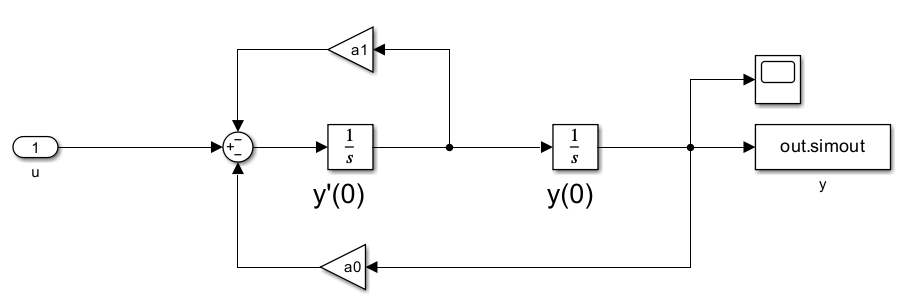
\includegraphics[width=1\textwidth]{scheme_system1.png}
	\caption{Структурная схема - система 2-го порядка}
\end{figure}
\newpage
\section{1-й эксперимент}
Так как мы решаем задачу для свободной составляющей движения системы, то учтём, что всегда будем подавать нулевой сигнал: $u = 0$:
$$
\ddot{y}_{free} + a_1\dot{y}_{free} + a_0y_{free} = 0
$$

Чтобы получить коэффициенты $a_0, a_1$, которые нам нужны для симуляции, будет достаточно вспомнить две вещи - сопоставление характерестического уравнения и теорему Виета для квадратного уравнения:
$$
\begin{aligned}
    \lambda^2 + a_1\lambda + a_0 = 0 \\
\end{aligned}
$$
Но так как мы заранее знаем корни, то решим обратную задачу с помощью теоремы Виета для нормированного случая:
$$
    \begin{aligned}
        \lambda_1 \cdot \lambda_2 = a_0 \\
        -(\lambda_1 + \lambda_2) = a_1 
    \end{aligned}
$$

В следующих эксперементах я не буду повторять эти выкладки, а сразу буду писать коэффициенты $a_0, a_1$.

Первая пара коэффициентов на подходе:
$$
\begin{aligned}
    \lambda_1 = -1, \lambda_2 = -1.5 \\
    a_0 = 1.5, a_1 = 2.5
\end{aligned}
$$
Для таких корней мы получим следующее аналитическое выражение свободного движения(воспользовались таблицей с модами):
$$
y_{free}(t) = c_1e^{-t} + c_2e^{-1.5t}
$$
Вычислим константы, используя начальные условия:
$$
    y(0) = c_1 + c_2 = 1 \tab \dot{y}(0) = -c_1 - 1.5c_2 = 0 
$$
$$
    c_2 = -2, \tab c_1 = 3
$$
В итоге получим:
$$
y_{free}(t) = 0.6e^{-t} + 0.4e^{-1.5t}
$$
На основании корневого критерия мы можем сказать, что асимптотически устойчива, так как все корни имеют отрицательную вещественную часть.

Получим следующиие результаты моделирования:
\begin{figure}[ht]
    \centering
    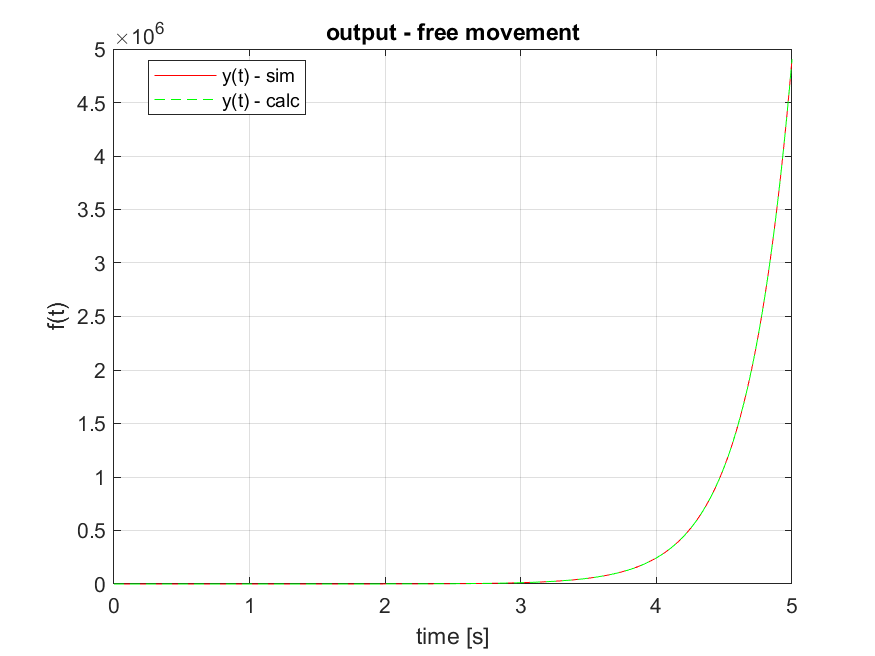
\includegraphics[width=0.8\textwidth]{output_task1_exp1.png}
	\caption{Симуляция - сопоставляем графики сигналов, аналитические и моделирования}
\end{figure}
\subsection{Выводы}
На основе эксперемента и аналитических расчётов мы можем увидеть, что данная система имеет \textbf{асимптотическую устойчивость}.


\newpage
\section{2-й эксперимент}
$$
\begin{aligned}
    \lambda_{3,4} = -0.6 \pm 4i \\
    a_0 = 0.36, a_1 = 1.2
\end{aligned}
$$
Для таких корней мы получим следующее аналитическое выражение свободного движения(воспользовались таблицей с модами):
$$
y_{free}(t) = e^{-0.6t}(c_1sin(4t) + c_2cos(4t))
$$
Вычислим константы, используя начальные условия:
$$
    y(0) = c_2 = 1 \tab \dot{y}(0) = 4c_1 - 0.6c_2 = 0 
$$
$$
    c_2 = 1, \tab c_1 = \frac{3}{20}
$$
В итоге получим:
$$
y_{free}(t) =  \frac{3}{20}e^{-0.6t}sin(4t) + e^{-0.6t}cos(4t)
$$
На основании корневого критерия мы можем сказать, что асимптотически устойчива, так как все корни имеют отрицательную вещественную часть.

Получим следующиие результаты моделирования:
\begin{figure}[ht]
    \centering
    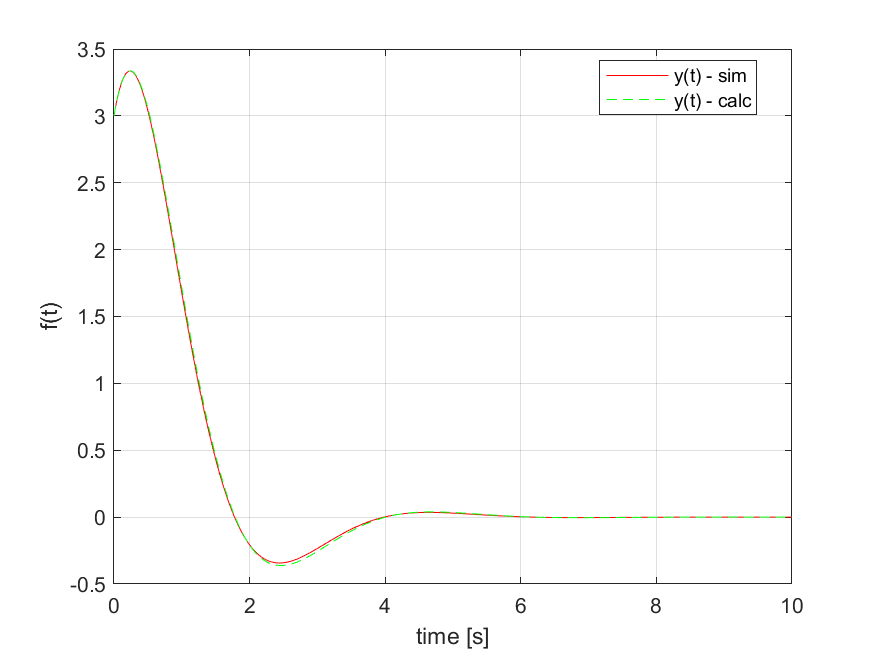
\includegraphics[width=0.8\textwidth]{output_task1_exp2.png}
	\caption{Симуляция - сопоставляем графики сигналов, аналитические и моделирования}
\end{figure}
\subsection{Выводы}
На основе эксперемента и аналитических расчётов мы можем увидеть, что данная система имеет \textbf{асимптотическую устойчивость}.


\newpage
\section{3-й эксперимент}
$$
\begin{aligned}
    \lambda_{5,6} = \pm 4i \\
    a_0 = 4, a_1 = 0
\end{aligned}
$$
Для таких корней мы получим следующее аналитическое выражение свободного движения(воспользовались таблицей с модами):
$$
y_{free}(t) = c_1sin(4t) + c_2cos(4t)
$$
Вычислим константы, используя начальные условия:
$$
    y(0) = c_2 = 1 \tab \dot{y}(0) = 4c_1 = 0 
$$
$$
    c_2 = 1, \tab c_1 = 0
$$
В итоге получим:
$$
y_{free}(t) =  sin(4t)
$$
На основании корневого критерия мы можем сказать, что система устойчива по Ляпунову, так как все корни имеют нулевую вещественную часть.

Получим следующиие результаты моделирования:
\begin{figure}[ht]
    \centering
    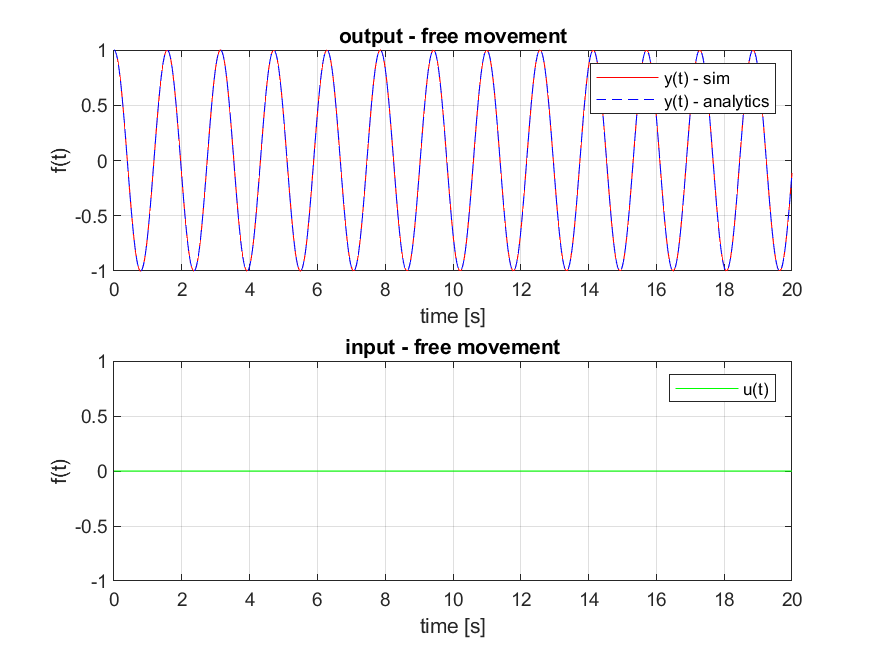
\includegraphics[width=0.8\textwidth]{output_task1_exp3.png}
	\caption{Симуляция - сопоставляем графики сигналов, аналитические и моделирования}
\end{figure}
\subsection{Выводы}
На основе эксперемента и аналитических расчётов мы можем увидеть, что данная система имеет \textbf{устойчивость по Ляпунову}.

\newpage
\section{4-й эксперимент}
$$
\begin{aligned}
    \lambda_{7,8} = 0.6 \pm 4i \\
    a_0 = 0.36, a_1 = -1.2
\end{aligned}
$$
Для таких корней мы получим следующее аналитическое выражение свободного движения(воспользовались таблицей с модами):
$$
y_{free}(t) = e^{0.6t}(c_1sin(4t) + c_2cos(4t))
$$
Вычислим константы, используя начальные условия:
$$
    y(0) = c_2 = 0.05 \tab \dot{y}(0) = 2c_1 + 3c_2 = 0 
$$
$$
    c_2 = 0.05, \tab c_1 = -\frac{3}{400}
$$
В итоге получим:
$$
y_{free}(t) =  e^{0.6t}(-\frac{3}{400}sin(4t) + \frac{1}{20}cos(4t))
$$
На основании корневого критерия мы можем сказать, что система неустойчива , так как хотя бы один корень имеет положительную вещественную часть.

Получим следующиие результаты моделирования:
\begin{figure}[ht]
    \centering
    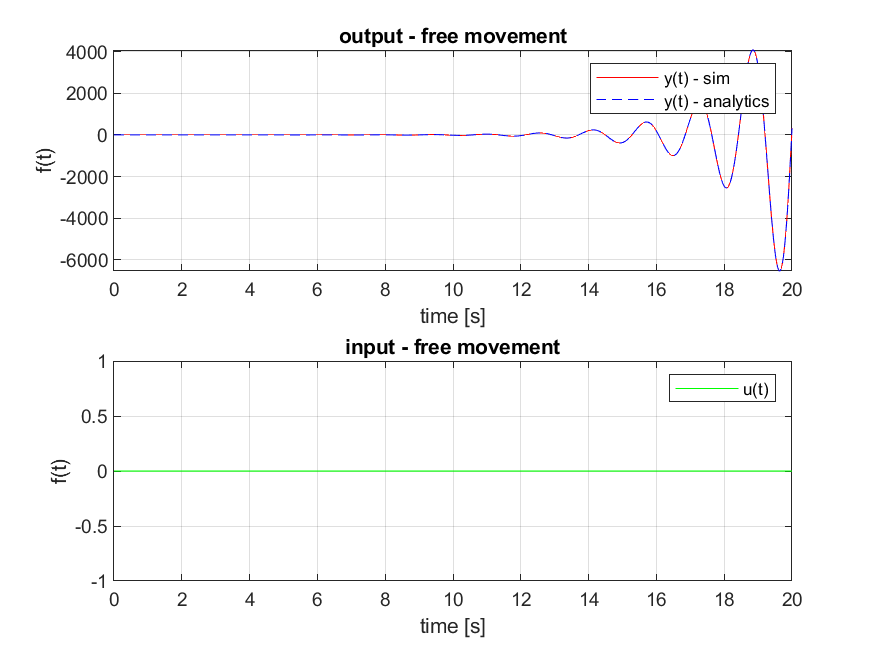
\includegraphics[width=0.8\textwidth]{output_task1_exp4.png}
	\caption{Симуляция - сопоставляем графики сигналов, аналитические и моделирования}
\end{figure}
\subsection{Выводы}
На основе эксперемента и аналитических расчётов мы можем увидеть, что данная система \textbf{неустойчива}.


\newpage
\section{5-й эксперимент}
$$
\begin{aligned}
    \lambda_9 = 1, \lambda_{10}=1.5 \\
    a_0 = 1.5, a_1 = -2.5
\end{aligned}
$$
Для таких корней мы получим следующее аналитическое выражение свободного движения(воспользовались таблицей с модами):
$$
y_{free}(t) = c_1e^{t} + c_2e^{1.5t}
$$
Вычислим константы, используя начальные условия:
$$
    y(0) = c_1 + c_2 = 0.05 \tab \dot{y}(0) = c_1 + 1.5c_2 = 0
$$
$$
    c_2 = -\frac{1}{10}, \tab c_1 = \frac{3}{20}
$$
В итоге получим:
$$
y_{free}(t) = \frac{3}{20}e^{t} + -\frac{1}{10}e^{1.5t}
$$
На основании корневого критерия мы можем сказать, что система неустойчива , так как хотя бы один корень имеет положительную вещественную часть.

Получим следующиие результаты моделирования:
\begin{figure}[ht]
    \centering
    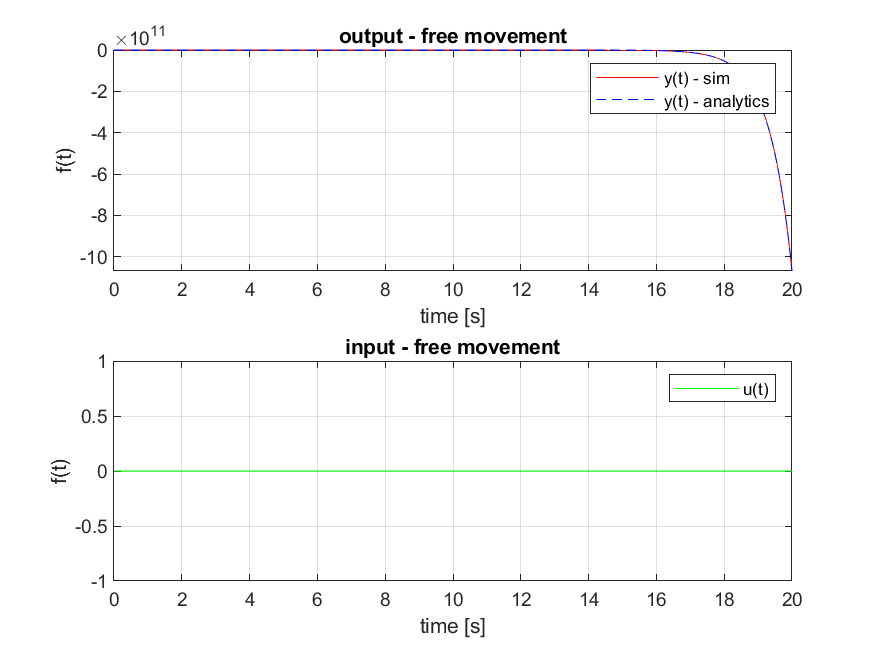
\includegraphics[width=0.8\textwidth]{output_task1_exp5.png}
	\caption{Симуляция - сопоставляем графики сигналов, аналитические и моделирования}
\end{figure}
\subsection{Выводы}
На основе эксперемента и аналитических расчётов мы можем увидеть, что данная система \textbf{неустойчива}.

\newpage
\section{6-й эксперимент}
$$
\begin{aligned}
    \lambda_{11} = -0.2, \lambda_{12}=0.2 \\
    a_0 = -0.04, a_1 = 0
\end{aligned}
$$
Для таких корней мы получим следующее аналитическое выражение свободного движения(воспользовались таблицей с модами):
$$
y_{free}(t) = c_1e^{-0.2t} + c_2e^{0.2t} 
$$
Вычислим константы, используя начальные условия:
$$
    y(0) = c_1 + c_2 = 0 \tab \dot{y}(0) = -0.2c_1 + 0.2c_2 = 0.1
$$
$$
    c_2 = \frac{1}{4}, \tab c_1 = -\frac{1}{4}
$$
В итоге получим:
$$
y_{free}(t) = -\frac{1}{4}e^{-0.2t} + \frac{1}{4}^{0.2t} 
$$
На основании корневого критерия мы можем сказать, что система неустойчива , так как хотя бы один корень имеет положительную вещественную часть.

Получим следующиие результаты моделирования:
\begin{figure}[ht]
    \centering
    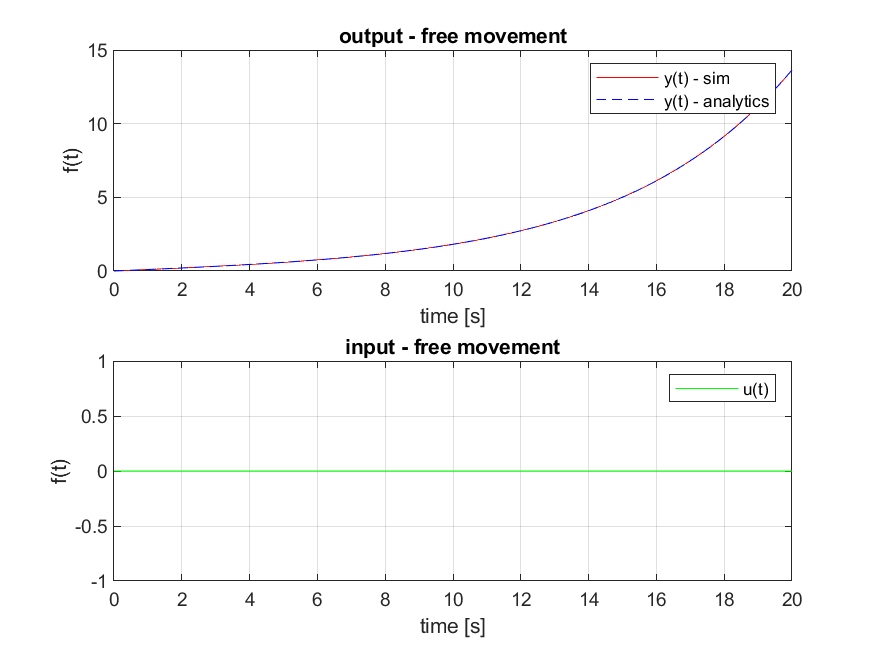
\includegraphics[width=0.8\textwidth]{output_task1_exp6.png}
	\caption{Симуляция - сопоставляем графики сигналов, аналитические и моделирования}
\end{figure}
\subsection{Выводы}
На основе эксперемента и аналитических расчётов мы можем увидеть, что данная система \textbf{неустойчива}.

\endinput